\section*{Ejercicios}

\begin{enumerate}

  \item Del circuito de la figura, obtener:
  \begin{itemize}
  \item Expresiones analíticas de las intensidades $i_1(t)$ e $i_2(t)$.
  \item Potencia disipada por todas las resistencias.
  \end{itemize}

  Datos: $\; e_g(t)=50\sqrt{2} \cos(1000\,t)$ V; \hspace{2mm}$i_g(t)=10$ A; \hspace{2mm}
$R_1=R_2=2\,\Omega$; \hspace{2mm} $R_3=7\,\Omega$; \hspace{2mm} $L_1=L_2=\qty{1}{\milli\henry}$; \hspace{2mm} $L_3=\qty{2}{\milli\henry}$
  \begin{center}
    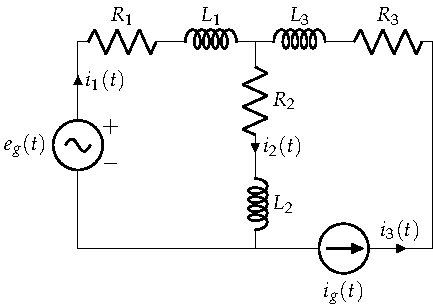
\includegraphics{../figs/ej18_BT2.pdf}
  \end{center}
  \emph{Sol.:\; 
    $i_1(t)= -5+5\sqrt{10}\cos(1000t-0.46) \,\si{\ampere};\; i_2(t)=
    5+5\sqrt{10}\cos(1000t-0.46) \,\si{\ampere};\; P_T=\qty{1300}{\watt}$}

\item En el circuito de la figura, determina:
  \begin{itemize}
  \item $u_R(t)$ y $u_L(t)$.
  \item Balance de potencias activas.
  \end{itemize}
  Datos:
  $\; e_a(t) = {3\sqrt{2} \sin(10^3 t)} \,\si{\volt};\;e_b(t) = {30\sqrt{2}
    \sin(10^4 t)}\,\si{\volt};\;R = \qty{30}{\ohm};\;L = \qty{3}{\milli\henry}$
  \begin{center}
    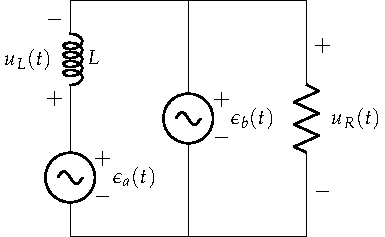
\includegraphics{../figs/superposicion2_ej.pdf}
  \end{center}

  \emph{Sol.:\;
    $u_R(t) = 30\sqrt{2}\sin(10^4 t)\,\si{\volt};\; u_L(t) = 3\sqrt{2}\sin(10^3
    t) - 30\sqrt{2}\sin(10^4 t)\,\si{\volt};\; P_R = \qty{30}{\watt};\; P_\epsilon =
    \qty{30}{\watt}$}

\item El circuito de la figura se encuentra en régimen
  permanente. Determinar analíticamente la expresión de $i(t)$, así
  como las potencias entregadas por los generadores y disipadas por
  las resistencias $R_1$ y $R_2$.

  Datos:
  $\; e_1(t) = \qty[parse-numbers=false]{50 \sin(1000 t)}{\volt};\;
  e_2(t) = \qty{30}{\volt};\;
  R_1 = \qty{6}{\ohm};\;
  R_2 = \qty{6}{\ohm};\;
  L = \qty{8}{\milli\henry};\;
  C = \qty{10}{\micro\farad}$

  \begin{center}
    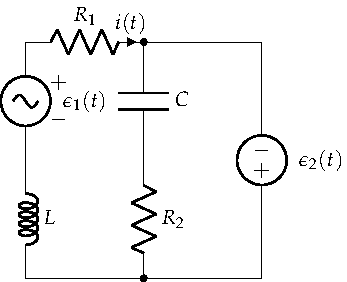
\includegraphics{../figs/superposicion1_ej.pdf}
  \end{center}
  \emph{Sol.:\;
    $i(t) = 5 + 5\sin(1000t - 0.9273){A};\; P_{R1} = {225}{W}; P_{R2}
    = {0}{W}; P_{\epsilon} = {225}{W}$}


\item Obtener el generador equivalente de Thévenin del circuito de la
  figura respecto de A y B. A partir de este generador, calcula la
  resistencia a colocar en A-B para obtener la máxima potencia,
  calculando esta potencia y la potencia entregada por el generador
  $\epsilon$.

  Datos:
  $\; \epsilon = \qty{54}{\volt};\; R_1 = R_4 = \qty{8}{\ohm};\;
  R_2 = R_3 = \qty{10}{\ohm}$

    \vspace{-1mm}
  \begin{center}
    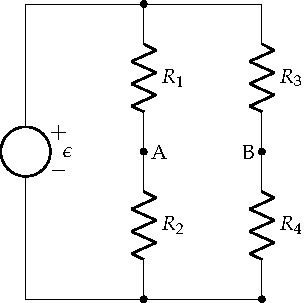
\includegraphics[height=4.75cm]{../figs/Thevenin2}
  \end{center}

    \vspace{-2mm}
    \emph{Sol.:\;
      $R_{AB} = \dfrac{80}{9}\,\si{\ohm}; \; P_R = \qty{1.0125}{\watt}; \;
      P_\epsilon = \qty{2.025}{\watt}$}

%%%%%%%%%%%%%%%%%%%%%%%%%%%

  \item Determinar el equivalente Thévenin del circuito de la figura
    entre los nudos A-B. ¿Qué resistencia habría que conectar en
    dichos terminales para transferir la máxima potencia? ¿Cuál sería
    dicha potencia?

    Datos: $\; R_1 = R_2 = \qty{4}{\ohm}$;\; $R_3 = \qty{2}{\ohm}$;\; $E = \qty{10}{\volt}$;\; $I_g = \qty{8}{\ampere}$

    \vspace{-3mm}
    \begin{center}
      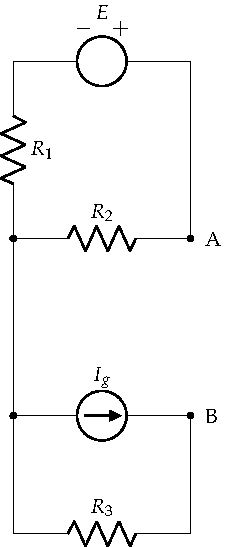
\includegraphics[height=9cm]{../figs/ej17_BT1.pdf}
    \end{center}

    \emph{Sol.:\;
      $\epsilon_{th}=5-16=\qty{-11}{\volt};\; R_{th}=\qty{4}{\ohm};\;
      R_L=\qty{4}{\ohm};\;P_{max}=\qty{7.56}{\watt}$}

%%%%%%%%%%%%%%%%%%%%%%%%%%%

  \item Obtener el generador equivalente de Thévenin del circuito de la figura respecto de A y B.
  
    Datos: $\; I_g=\qty{10}{\ampere};\; R_1=\qty{1}{\ohm};\; \alpha=5$
    \begin{center}
      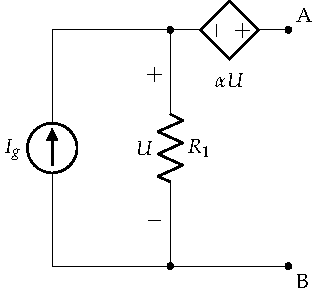
\includegraphics[height=4.75cm]{../figs/Thevenin1.pdf}
    \end{center}

    \emph{Sol.:\; $\epsilon_{th}=\qty{60}{\volt};\; R_{th}=\qty{6}{\ohm}$}

%%%%%%%%%%%%%%%%%%%%%%%%%%%

    % \item En el circuito de la figura, se debe calcular el equivalente de Norton entre terminales A-B.

    % \begin{minipage}{0.6\linewidth}
    %   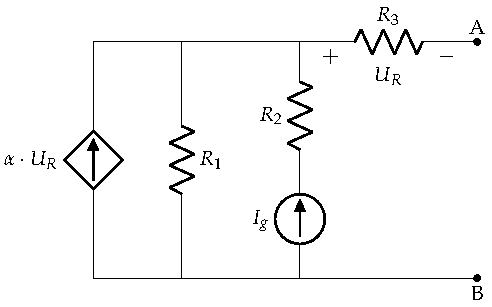
\includegraphics[height=4.75cm]{../figs/BT1_ej19_enunciado.pdf}
    % \end{minipage}
    % \begin{minipage}{0.4\linewidth}
    %   Datos:
    %   \vspace{2mm}
      
    %   $R_1 = R_3 = \qty{1}{\ohm}$\\[1mm]
    %   $R_2 = \qty{2}{\ohm}$\\[1mm]
    %   $\alpha = 0.5\,\si{\ohm}^{-1}$\\[1mm]
    %   $I_g = \qty{6}{\ampere}$
    % \end{minipage}

    % \emph{Sol.:\; 
    %   $I_N = \qty{4}{\ampere};\; R_N = \dfrac{3}{2}\,\si{\ohm}$}
      
%%%%%%%%%%%%%%%%%%%%%%%%%%%

  \item En el circuito de la figura, calcular:
    \begin{itemize}
    \item La corriente del generador equivalente de Norton respecto de
      A y B, $I_N$.
    \item La resistencia del generador equivalente de Norton respecto
      de A y B, $R_N$.
    \item La resistencia de carga que se debe conectar entre A y B
      para conseguir la máxima potencia disponible, y el valor de esta
      potencia.
    \end{itemize}
    Datos:
    $\; R = \qty{1}{\ohm};\; \epsilon_g = \qty{10}{\volt};\; \alpha = \qty{2}{\ohm};\; \beta = 1$

    \begin{center}
      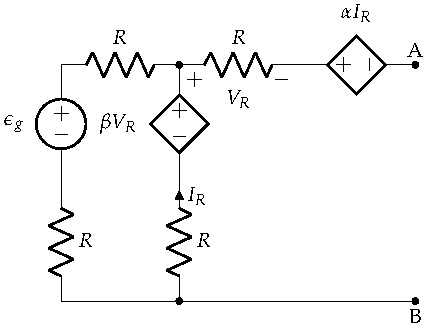
\includegraphics[height=5.5cm]{../figs/norton.pdf}
    \end{center}

\emph{Sol.:\;
  $I_N=\dfrac{10}{3}\,\si{\ampere};\; R_N=\qty{3}{\ohm};\; R_L=\qty{3}{\ohm};\;
  P_L=\dfrac{25}{3}\,\si{\watt}$}

\item   Obtén el equivalente de Thévenin del circuito de la figura
  respecto de A y B, así como la impedancia a conectar en estos terminales para obtener la máxima potencia posible.

Datos: $\; \overline{\epsilon}_g = \qty[parse-numbers=false]{12 - 16j}{\volt};\;
  \overline{Z}_1 = \qty[parse-numbers=false]{1 - j}{\ohm};\;
  \overline{Z}_2 = \qty[parse-numbers=false]{1 + j}{\ohm};\;
  \overline{Z}_3 = \qty[parse-numbers=false]{5 + 3j}{\ohm};\;
  \alpha = 2 $
  
\begin{center}
  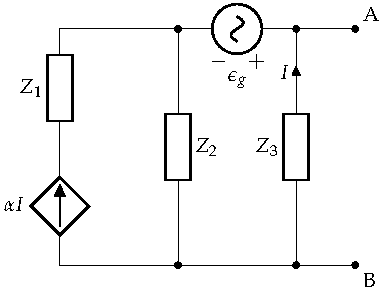
\includegraphics{../figs/Thevenin4}
\end{center}

\emph{Sol.:\;
  $ \overline{\epsilon}_{th} = 11.66\phase{\ang{-59.04}}\,\si{\volt};\;
  \overline{Z}_{th} = 0.64 + 0.52j\,\si{\ohm};\; \overline{Z}_L = 0.64-0.52j\,\si{\ohm};\; P_L = \qty{53.11}{\watt}$}

\item Obtén el equivalente de Thévenin del circuito de la figura respecto de A y B. A partir de este equivalente, calcula la impedancia a colocar en AB para obtener la máxima potencia, calculando también dicha potencia.

\begin{minipage}{0.5\textwidth}
\begin{center}
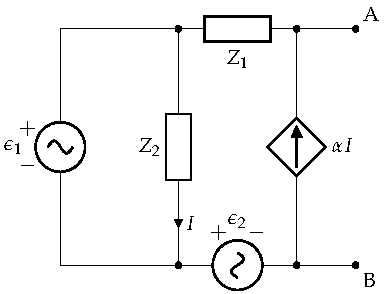
\includegraphics{../figs/Thevenin5}
\end{center}
\end{minipage}
\begin{minipage}{0.5\textwidth}
\hspace{20mm}Datos:
  \begin{align*}
    \overline{\epsilon}_1 &= \SI[parse-numbers=false]{10\phase{0}}{\volt}\\
    \overline{\epsilon}_2 &= \SI[parse-numbers=false]{10j}{\volt}\\
    \overline{Z}_1 &= \SI[parse-numbers=false]{4 - 3j}{\ohm}\\
    \overline{Z}_2 &= \SI[parse-numbers=false]{3 + 4j}{\ohm}\\
    \alpha &= 2
  \end{align*}
\end{minipage}

\vspace{2mm}
\emph{Sol.:\; $
  \overline{\epsilon}_{th} =  10 - 10j \,\si{\volt};\;
  \overline{Z}_{th} = 4 - 3j \,\si{\ohm};\; \overline{Z}_L = 4 + 3j\,\si{\ohm};\; P_L = \qty{12.5}{\watt}
  $}


\end{enumerate}

%%% Local Variables:
%%% mode: latex
%%% TeX-master: "enunciados_ejercicios_TC"
%%% ispell-local-dictionary: "castellano"
%%% End:
